\title{Optimisations for finite state Mealy automata}
\author{
        Aleksander Mendoza \\
                Department of Mathematics and Computer Science\\
        Adam Mickiewicz University\\
        Poznan, \underline{Poland}         
}
\date{\today}

\documentclass[12pt]{article}
\usepackage{tikz}
\usepackage[utf8]{inputenc}
\usepackage[T1]{fontenc}
\usepackage{lmodern}
\usepackage{amsfonts}
\usepackage{mathrsfs}
\usepackage{centernot}
\usepackage{listings}
\usepackage{mathtools}
\usepackage{xcolor}
\usepackage{amsmath}
\usepackage{amssymb}

\begin{document}
\maketitle
\lstset{
	basicstyle=\ttfamily,
	mathescape
}

\section{Introduction}
Standard definition of Mealy machine is provided as $(Q,q_0,\Sigma,\Gamma,\delta,G,F)$ where $Q$ is set of states, $q_0 \in Q$ is the initial state, $\Sigma$ and $\Gamma$ are respectively input and output alphabets, $\delta: Q \times \Sigma \rightarrow Q$ is the transition function , $G: Q \times \Sigma \rightarrow \Gamma$ it specifies output associated with each transition and $F$ is the set of accepting states. Finite state automaton is defined similarly as $(Q,q_0,\Sigma,\delta, F)$ but it doesn't have any output. It's possible to extend both machines to non-deterministic models by adding $\epsilon$ to transition and/or output functions as in 
$\delta: Q \times (\Sigma \cup \{\epsilon\})\rightarrow Q$ and $G: Q \times (\Sigma \cup \{\epsilon\})\rightarrow (\Gamma \cup \{\epsilon\})$.  We can show that introducing non-determinism this way is equivalent to defining it as $\delta: Q \times (\Sigma \cup \{\epsilon\})\rightarrow P(Q)$ for finite state automata (and $\delta: Q \times (\Sigma \cup \{\epsilon\}) \rightarrow P(Q \times \Gamma)$ for Mealy machines) but in our case, just adding epsilon is enough and will make things simpler later.  \textcolor{red}{Dowód dodam potem.} You can treat finite state machines as predicates on formal languages. For instance if $P$ is an automaton, then $\forall_{x\in \Sigma^*} P(x) \iff P \textrm{ accepts }x$. Mealy machines on the other hand, can be interpreted as relations on languages. Let's say $M$ is a Mealy machine, then $\forall_{x\in\Sigma^*, y \in \Gamma^*} M(x,y) \iff M \textrm{ produces } y \textrm{ as one of it's outputs, on input } x$. So in a sense, $P$ is equivalent to some subset of $\Sigma^*$, while $M$ is equivalent to some subset of $\Sigma^* \times \Gamma^*$. If additionally $M$ is a function ( it holds that $\forall_{x\in\Sigma^* , y,z \in \Gamma^* } M(x,y) \wedge M(x,z) \implies y=z$ ), then we can write $M(x)=y$ instead of $M(x,y)$. It's important to remember that there  might exist many different automata inducing the same language or relation on languages. Therefore we shall write $P_0 = P_1$ to mean $\forall_{x\in\Sigma^*} P_0(x) \iff P_1(x)$ even when $P_0$ and $P_1$ have different structures. Similarly $M_0 = M_1$ when $\forall_{x \in \Sigma^* , y\in\Gamma^*}M_0(x,y) \iff M_1(x,y)$.  We define two projections for Mealy machines: 
\begin{itemize}
	\item input projection $\pi_0(M) = P$ such that $\forall_{x\in\Sigma^*} (\exists_{y\in\Gamma^*}M(x,y) ) \iff P(x) $
	\item output projection  $\pi_1(M) = P$ such that $\forall_{y\in\Gamma^*} (\exists_{x\in\Sigma^*}M(x,y) ) \iff P(y) $
\end{itemize} 
Deterministic and non-deterministic automata are equivalent in their power to recognise formal languages, however non-deterministic Mealy machines have more expressive power to relate two formal languages with each other. Let's consider several cases with help of pumping lemma. 

\paragraph{Pumping lemma for regular languages}
If $L$ is a regular language then there exists $p\ge1$  such that for all $l \in L$ where $\vert l \vert \ge p$ , can be decomposed to $l = xyz$ that satisfy the following conditions:
\begin{itemize}
	\item $\vert y \vert \ge 1$ 
	\item $\vert xy \vert \le p$ 
	\item $\forall_{n\in \mathbb{N}}  xy^nz \in L$ 
\end{itemize}

\paragraph{Deterministic single-output Mealy machines} Determinism guarantees us that for given machine $M$, the relation $M \subset \Sigma^* \times \Gamma^*$ is in fact a function $M \subset \Sigma^* \rightarrow \Gamma^*$. For any input $x \in \Sigma^*$, there exists only one output $y\in \Gamma^*$ such that $M(x,y)$. Moreover because $G: Q \times \Sigma \rightarrow \Gamma$ always returns exactly one element from $\Gamma$, we can be sure that $\vert x\vert = \vert y\vert$. We can apply pumping lemma to both input and output projection of $M$. We can also go further and fuse both $\Sigma$ and $\Gamma$ using Cantor's pairing function into a new alphabet $\Sigma \times \Gamma$ and then apply pumping lemma to it. Another important feature is that prefixes must match: \\
$\forall_{x,y\in \Sigma^*} \exists_{a \in \Gamma^* } M(xy)=M(x)a$ \\
This is a very problematic restriction. It implies that relation \\
$M(x) = \begin{cases}
0^{\vert x \vert} & \mbox{if } \vert x \vert \mbox{ is multiple of 2}   \\
1^{\vert x \vert}& \mbox{otherwise} 
\end{cases}$ \\
is not possible, because $M(a) = 1$, $M(aa) = 00$  for $a \in \Sigma$ and $0,1 \in \Gamma$. However, it is worth noticing that relations: \\
$M_0(x) = \begin{cases}
0^{\vert x \vert} & \mbox{if } \vert x \vert \mbox{ is multiple of 2}   \\
\mbox{ reject otherwise} 
\end{cases}$ \\
and  \\
$M_1(x) = \begin{cases}
1^{\vert x \vert} & \mbox{if } \vert x \vert \mbox{ is not multiple of 2}   \\
\mbox{ reject otherwise} 
\end{cases}$ \\
are valid. The class of relations defined by this model is not closed under union.

\paragraph{Deterministic multi-output Mealy machines} This model is defined as above except that $G: Q \times \Sigma \rightarrow \Gamma^*$. This breaks the guarantee that $\vert x\vert = \vert y\vert$. Now $y$ can be of any length. However, you can still apply pumping lemma to both projections of $M$. You just cannot apply it to fused alphabet $\Sigma \times \Gamma$. Moreover, the prefix restriction still holds: \\
$\forall_{x,y\in \Sigma^*} \exists_{a \in \Gamma^* } M(xy)=M(x)a$ \\


\paragraph{Functional Mealy machines} They are defined in a very different way. They can write to multiple   tapes. Output function becomes $G: Q \times \Sigma \times T \rightarrow \Gamma^*$ where $T$ is a finite set of tapes. $F$ is no longer a set but a function $F: Q \rightarrow T \cup \{\emptyset\}$. This model works by reading consecutive input characters $s \in \Sigma$ , and transitioning from state $q\in Q$ to $\delta(q,s)$. On each transition automaton writes  $G(q,s,t)$ to every tape $t \in T$. When input reaches end and automaton halts in state $q$, the returned output should be taken from $F(q)$. In cases when $F(q) = \emptyset$ , the automaton rejects. This model is still deterministic but multiple tapes allow it to break the rule of matching prefixes.


\paragraph{Non-deterministic Mealy machines} This model allows for greatest flexibility. $M \subset \Sigma^* \times \Gamma^*$ does not have any restrictions apart from the requirement that both input and output language must be regular. Furthermore, we can use epsilons to associate one input with multiple outputs. In fact, there could be infinitely many of them if epsilons create a loop at some point. 



\paragraph{Classes of language relations} As mentioned above, Mealy machines represent some class of relations on languages. A relation $R \subset \Sigma^* \times \Gamma^*$ is decidable if there exists some Turing machine that works on alphabet $\Sigma \cup \Gamma$ and accepts all strings in $R$ while also rejects all strings from $\overline{R}$ (we can use arbitrary way to encode pairs of strings). Of course not all relations are decidable. The most trivial example of undecidable relation is $(x,y)  \in \Sigma^* \times \{0,1\}$ where  $x$ encodes some Turing machine, and $y$ is in relation with $x$ iff $x$ halts on $y$. While Turing machines are capable of "recognizing" pairs of strings, Mealy automata can be used to "generate" the right-side element of pair for any given left-side element of pair. However, in principle both "generation" and "recognition" are just different ways to see the same phenomenon. Anything that can be generated with mealy machines can be recognized by some Turing machine. 

\paragraph{} Let's say that we are given non-deterministic Mealy machine $M$ and input $(x,y) \in \Sigma^* \times \Gamma^*$ . The problem whether $(x,y) \in M$ is decidable, because we can simulate all non-deterministic branches of computation and reject them as soon as the length of total accumulated output equals or exceeds length of $y$. There are only finitely many strings in $\Gamma^*$ shorter or equal $y$, so we can visit all of them in finite time. Also, at any step the computation of Mealy automaton can split into only finite number of new non-deterministic branches. 

\paragraph{} This proves that simulation of non-deterministic Mealy machines is computable. For all deterministic models the proof is even simpler. Unfortunately is doesn't work the other way around. It's not possible in general case to build Mealy machine equivalent to given Turing machine. The proof is very simple - languages accepted and generated by Mealy machines are regular. 

\paragraph{} Apart from input and output languages being regular themselves, there are also limitations to how the relation on those languages can be structured. There exists a relation $ R \subset \Sigma^* \times \Gamma^*$
such that both $\pi_0(R)$ and $\pi_1(R)$ are regular, but despite this there is no non-deterministic Mealy automaton capable of deciding it. Proof is simple. Let $s,t\in \Gamma^*$ such that $s\ne t$ and let $R:\Sigma^* \rightarrow \Gamma^*$ such that: \\
$R(x) = \begin{cases}
t & \mbox{if }  x  \mbox{ is a valid description of Turing machine that halts on } x   \\
s & \mbox{otherwise} 
\end{cases}$ \\
Notice that $\pi_0(R) = \Sigma^*$ and $\pi_1(R) = \{s,t\}$ and both are regular. Moreover this relation is not only undecidable by Mealy machines but also not decidable by any computation model at all.

\subparagraph{Pair encodings} We can actually tell even more about the class of all relations generated by Mealy machines, but for this we need a more precise encoding for pairs of strings:
\begin{itemize}
	\item Separated pairs - Given two strings $s \in \Sigma^*$ and $t \in \Gamma^*$ we encode a pair $(s,t) \in \Sigma^* \times \Gamma^*$ as $w \in (\Sigma \cup \Gamma \cup \{\#\})^*$ where $w=s\#t^{-1}$,  $\# \notin \Sigma \cup \Gamma$ and $t^{-1}$ means "reverse of $t$". For given $R \subset \Sigma^* \times \Gamma^*$ we denote encoding of $R$ as $\mathbb{S}_\#(R) = \{w\in (\Sigma \cup \Gamma \cup \{\#\})^*: w=s\#t^{-1} \wedge (s,t) \in R \}$. Notice that for any $R$, the encoding $\mathbb{S}_\#(R)$ is unique. We say that relation $R$ is regular if there exists finite state automaton $P$ such that  $\forall_{s,t} R(s,t) \iff P(s\#t^{-1})$. Similarly $R$ is context-free if $P$ is a push-down automaton. Also, it's worth pointing out that the class of all relations is a proper subset of class of all formal languages. That's because of the restriction that every string must contain exactly one $\#$ (Given formal language $R$ over alphabet $\Theta$ you might not always be able to find isomorphism between $\Theta$ and $\Sigma \cup \Gamma \cup \{\#\}$ such that $\#$ appears in every string in $R$ exactly once).
	
	\item Interleaved pairs - Given two strings $s \in \Sigma^*$ and $t \in \Gamma^*$ we encode a pair $(s,t) \in \Sigma^* \times \Gamma^*$ as $w \in (\Sigma \cup \Gamma)^* $ where $\Sigma$ and $\Gamma$ \underline{are disjoint} , $w$ equals $s$ when you remove from $w$ all characters belonging to $\Gamma$ and similarly $w$ equals $t$ when you remove from $w$ all characters belonging to $\Sigma$. If $R \subset  \Sigma^* \times \Gamma^*$ then we denote $\mathbb{I}(R) \subset (\Sigma \cup \Gamma)^*$ as interleaved encoding of $R$. An example:\\
	Let $\Sigma = \{0,1,2\}$, $\Gamma = \{3,4,5\}$. Then pair $(001,354) \in R$ could be encoded as $030154 \in \mathbb{I}(R)$ or as $001354 \in \mathbb{I}(R)$, or $354001 \in \mathbb{I}(R)$ and so on. \\
	You can see that every pair does not have a single encoding but rather an entire class of strings becomes a valid encoding. We will say that for given encoding $\mathbb{I}(R) \subset (\Sigma \cup \Gamma)^*$ a pair $(x,y)$ belongs to $R \subset \Sigma^* \times \Gamma^*$ iff there exists at least string $\mathbb{I}(R)$ that encodes $(x,y)$. Formally $(x,y) \in R \iff \exists_{w\in\mathbb{I}(R)} w - \Sigma = y \wedge w - \Gamma = x$ where $w-X$ denotes operation of removing from string $w$ all characters from set $X$. Notice that for given $R$ there might exist multiple equivalent sets $\mathbb{I}(R)$ that encode it. Analogically to separated encoding, $R$ is regular if there exists regular $\mathbb{I}(R)$, and it is context-free if there exists context-free $\mathbb{I}(R)$. Also, it's worth pointing out that class of interleaved relations is exactly equal to class of all formal languages, because for any given formal language over alphabet $\Sigma$ you can always split $\Sigma$ into two disjoint subsets $\Sigma_0$ and $\Sigma_1$, and then interpret every string in $\Sigma^*$ as some pair in $\Sigma_0^* \times \Sigma_1^*$.
\end{itemize}
 
 \subparagraph{} From now on, we will use $\mathbb{M}_1$ to refer to class of relations decidable by single-output, $\mathbb{M}_\infty$ for multi-output , $\mathbb{M}_\rightarrow$ for functional and $\mathbb{M}$ for non-deterministic Mealy machines. $\mathbb{REG}$ will be used to describe class of regular languages  and $\mathbb{CFG}$ for context-free languages. For given class of relations X, we will write $\mathbb{I}(X)$ to denote class of formal languages that encode relations from $X$. Formally $L  \in X \iff \mathbb{I}(L)  \in \mathbb{I}(X)$ where $L \subset \Sigma^* \times \Gamma^*$ and $\mathbb{I}(L) \subset (\Sigma \cup \Gamma)^*$. 
 
For encoding  $\mathbb{S}_\#$ it works analogically, except there is one important detail. We need to make it precise what "class of languages" stands for. A formal language is just a set of strings over some alphabet. A class of formal languages therefore is a set of sets of strings over some alphabet. There is no restriction that forces all the languages in one class to share common alphabet. In many books and papers this detail is overlooked or left implicit. Here, however, the separator character $\#$ requires us to be explicit about the alphabets and for this reason we need clear distinction between homogeneous and heterogeneous classes. 

 \subparagraph{Homogeneous and heterogeneous classes}  Formal language over finite alphabet $\Sigma$ is a subset of $\Sigma^*$. Homogeneous class of formal languages $X$ is defined as set of formal languages such that all members $L \in X$ share the same alphabet. Formally $X \subset\mathcal{P}(\Sigma^*)$ On the other hand, in a heterogeneous class of formal languages every member language could potentially use different alphabet. There are two rules of formation for such classes:
 \begin{enumerate}
	\item every homogeneous class is also a heterogeneous class
	\item if $Y$ is set (of any cardinality) of  heterogeneous classes then union	\[
	\mathop{\bigcup} Y  
	\] is a heterogeneous class
 \end{enumerate} 
An important thing worth noticing is that many heterogeneous classes can be seen as homogeneous classes. Suppose there are two homogeneous formal languages $X_\Sigma \subset \Sigma^*$ and  $X_\Gamma \subset \Gamma^*$. However obviously if $\Sigma$ and $\Gamma$ are finite sets then $\Sigma \cup \Gamma$ is a finite set too. Therefore the union $X_\Sigma \cup X_\Gamma$ could be a heterogeneous class derived from second rule of formation or it could be a  homogeneous class $X_\Sigma \cup X_\Gamma \subset (\Sigma \cup \Gamma)^*$. Unfortunately not all heterogeneous classes can be treated this way. The problem lies in the requirement that alphabet is finite, while the second rule of formation would allow us to have in total infinitely many disjoint alphabets (so the union of alphabets would be infinite as a result).  We can go even further and define universum $\mathcal{U}$ as the set of all finite sets, and treat it as set of all possible alphabets. Then we can define formal language universum $\top$ which is the heterogeneous class of all formal languages given by \[
\top = \bigcup_{\Sigma \in \mathcal{U}} \mathcal{P}(\Sigma^*) 
\]
Notice that $\mathbb{REG}$ and $\mathbb{CFG}$ are both heterogeneous classes in universum $\mathbb{CFG}, \mathbb{REG} \subset \top$. 

We can also extend notion of homogeneous and heterogeneous classes to relations on languages. Homogeneous class of relations $X$ over alphabets $\Sigma$ and $\Gamma$ is a subset $X \subset \mathcal{P}(\Sigma^* \times \Gamma^*)$. Heterogeneous classes of relations are constructed using analogical rules of formation as classes of languages.

After settling precise definition of classes of formal languages we can go back to the problem of separated relations. Given a class of relations $X$ (homogeneous or not), the separator character $\#$ need \underline{not} be unique or universal for all languages that are members of \underline{heterogeneous} $\mathbb{ S}(X)$. If we require all the classes to be homogeneous we can explicitly specify it as $\mathbb{ S}_\#(X)$ where $\#$ is separator character used universally by all the classes (we require that $X$ is homogeneous itself). Formally:
\begin{itemize}
	\item $\mathbb{ S}_\#(X) $ is defined as $ R \in X \iff \mathbb{ S}_\#(R) \in \mathbb{ S}_\#(X)  $ where $X$ is a homogeneous  class of relations on formal languages
	\item Given $R \subset \Sigma^* \times \Gamma^*$, $\mathbb{ S}(R)$  is defined as $\forall_{\# \notin \Sigma \cup \Gamma} \mathbb{ S}_\#(R) \in \mathbb{ S}(R)$ 
	\item $\mathbb{ S}(X)$ is defined as  $R \in X \iff \mathbb{ S}(R) \in \mathbb{ S}(X)  $
\end{itemize} 
 Notice that for any two characters $a,b \notin \Sigma \cup \Gamma$ the languages $\mathbb{S}_a(R)$ and $\mathbb{S}_b(R)$ are isomorphic (the only difference is substitution of separator $a$ for separator $b$ or vice versa). 
 
\subparagraph{Hierarchy of classes} Obviously $\mathbb{M}_0 \subsetneq \mathbb{M}_{\infty}  \subsetneq \mathbb{M}_{\rightarrow}  \subsetneq \mathbb{M} $, but now when we have all the necessary tools and definitions we  can show further the correlations between Mealy machine models and classes of relations and their encodings:
 \begin{enumerate}


\item $\mathbb{S}(\mathbb{M}) \subset \mathbb{CFG}$ Class of relations generated by non-deterministic Mealy machines is a proper subclass of context-free separated relations. The proof idea is simple: \\
Given non-deterministic Mealy automaton $M$ on alphabets $\Sigma$ and $\Gamma$ we build context-free grammar with non-terminal alphabet $V$ and terminal alphabet $\Sigma \cup \Gamma \cup \{\#\}$. For any $(q,s,q') \in \delta \subset Q \times (\Sigma \cup \{\epsilon\}) \rightarrow Q$ and $(q,s,s') \in G \subset Q \times (\Sigma \cup \{\epsilon\}) \rightarrow (\Gamma \cup \{\epsilon\})$ we generate context-free rule $V_q \rightarrow s V_{q'} s'$.  We also add initial rule $S \rightarrow V_{q_0}$ where $q_0$ is initial state of $M$. At the end for every $q \in F$ we add rules $V_q \rightarrow \#$. If for any given string $w \in \Sigma \cup \Gamma \cup \{\#\}$ there exists a valid derivation tree in such CFG, then we can be sure that there exists a corresponding path in $M$ that leads from initial to final state and produces $w$ along the way. \\
Unfortunately it's not true that any context-free relation can be generated by Mealy machines (the proof is quite obvious). $ \mathbb{CFG} \not\subset \mathbb{S}(\mathbb{M})$

\item $\mathbb{REG} \cap \mathbb{S}(\mathbb{M}) \subsetneq \mathbb{S}(\mathbb{M})$ Class of relations generated by non-deterministic Mealy machines is a proper superclass of regular separated relations. We need to prove that $\mathbb{REG} \cap \mathbb{S}(\mathbb{M}) \subset \mathbb{S}(\mathbb{M})$ and $\mathbb{S}(\mathbb{M}) \not\subset \mathbb{REG} \cap \mathbb{S}(\mathbb{M})$. The first case is trivial. The second is much more tedious. Here is its proof: \\
Assume to the contrary that for any $M \in \mathbb{M}$, we can find finite state automaton $P$ that recognizes  $\mathbb{S}(M)$. Let's take the first projection of $\mathbb{S}(M)$ given by 
$\Pi_0 = \{s \in \Sigma^* : \exists_{t\in\Gamma^*} s\#t \in M\}$. We can always find such automaton $P'$ that is a sub-automaton of $P$ (has some states and edges removed, no new edges or states are added, and additionally accepting states are changed) and accepts $\Pi_0$. Because every string $s \in  \mathbb{S}(M)$ must contain exactly one $\#$, we can deduce that once $P'$ accepts, some transition labeled with $\#$ must take you to some new state that is in $P$ but not in $P'$ and it's not possible to ever go back to any state in $P'$. In other words, accepting states of $P'$ mark the states in $P$ with outgoing $\#$-edges. There can only by finitely many such $\#$-states and each of them has exactly one (for deterministic FSA) $\#$-edge. We can divide $\Pi_0$ into congruence classes based on which accepting state in $P'$ they end up in. The most important implication that follows from it is that we can also divide $ \mathbb{S}(M)$ based on this criterion - given $(s_0,t_0),(s_1,t_1) \in \mathbb{S}(M)$ the two relations are congruent iff $s_0$ and $s_1$ are congruent too. Because $P'$ has only finitely many accepting states, there can be only finitely many congruence classes. The property of such congruence is that if $(s_0,t_0)$ is congruent with $(s_1,t_1)$ then $(s_0,t_1),(s_1,t_0)\in M$ (because both $s_0$ and $s_1$ reached the same $\#$-state and both $s_0\#$ and $s_1\#$ transitioned over the same $\#$-edge, so at that point the automaton lost all memory about whether the left-side element of pair was $s_0$ or $s_1$ and it will have to behave the same way in both cases and accept the same right-side elements of pair). Obviously this property does not hold for all non-deterministic Mealy automata in general. They might require infinitely many congruence classes to make such property hold.

\item $\mathbb{REG} \cap \mathbb{S}(\mathbb{M}) \not\subset \mathbb{S}(\mathbb{M}_\rightarrow)$  This one is quite obvious. $\mathbb{S}(\mathbb{M}_\rightarrow)$ only contains relations that are  functions while $\mathbb{REG} \cap \mathbb{S}(\mathbb{M})$ contains any relations.  

\item $\mathbb{S}(\mathbb{M}_\rightarrow)\not\subset\mathbb{REG} \cap\mathbb{S}(\mathbb{M})$ To prove this one we can reuse proof of $\mathbb{REG} \cap \mathbb{S}(\mathbb{M}) \subsetneq \mathbb{S}(\mathbb{M})$. Every finite state automaton from class of regular separated relations $\mathbb{REG} \cap \mathbb{S}(\mathbb{M})$ contains finitely many $\#$-states. However, look at this counter-example of $M \in \mathbb{M}_\rightarrow$ given by: \\
$M(x) = \begin{cases}
0^{\vert x \vert} & \mbox{if }  x  \in 1^*   \\
\mbox{reject} & \mbox{otherwise} 
\end{cases}$ \\
There are infinitely many relations of form $(1^n,0^n)$  generated by $M$ and for none of them it holds that if $(1^n,0^n)$ is congruent with $(1^m,y^m)$ then $(1^n,0^m), (1^m,y^n)  \in M$. This leads to contradiction.


\item $\mathbb{REG} = \mathbb{I}(\mathbb{M})$  Class of relations generated by non-deterministic Mealy machines is exactly equal to class of regular interleaved relations. 

First we prove $\mathbb{I}(\mathbb{M})  \subset \mathbb{REG} $. The proof is constructive and the idea is simple - you just "flatten" input and output together. Let $M \in \mathbb{M}$ be non-determinisitc Mealy relation in $\Sigma^* \times \Gamma^*$ such that $\Sigma \cap \Gamma = \emptyset$. We will build a finite state automaton $P \subset (\Sigma \cup \Gamma)^*$ such that its recognized language is equivalent to one of possible interleaved encodings $ P = \mathbb{I}(M)$ . For every state $m \in Q_M$ and alphabet character $s \in \Sigma \cup \{\epsilon\}$ there is transition $m' = \delta_M(m,s)$ and output $s' = G_M(m,s) \in \Gamma \cup \{\epsilon\}$. Then in $P$ there shall exist $(p_m,s,p_{ms}), (p_{ms},s',p_{m'}) \in \delta_P \subset Q_P \times (\Sigma \cup \Gamma \cup \{\epsilon\}) \rightarrow Q_P$. So for every transition in $\delta_M$ and output in $G_M$ there is corresponding state in $Q_P$ that simulates it. First $P$ reads some input $\Sigma$ then goes to a new state that expects to read output $\Gamma$. Such construction implements a particular encoding of $\mathbb{I}(M)$ - such that exactly corresponds to order of reading and printing events in $M$. To finalize this construction we need to specify that for every accepting state $m \in F_M$ there is a corresponding accepting state $p_m$ and for initial state $m_0$ there is also initial state $p_{m_0}$. 
 
 Now we prove $\mathbb{REG} \subset \mathbb{I}(\mathbb{M})$ . Suppose $P$ is some deterministic finite automaton over alphabet $\Sigma$. We can always split $\Sigma$ into $\Sigma_0$ and $\Sigma_1$ such that $\Sigma_0 \cap \Sigma_1 = \emptyset$ and $\Sigma_0 \cup \Sigma_1 = \Sigma$. Every string in $\Sigma$ becomes at the same time also some interleaved pair in $\Sigma_0 \times \Sigma_1$. We attempt to build non-deterministic Mealy machine $M$ that accepts every such pair, except that this time for convenience (as both models are equivalent) we define transition function as $\delta_M : Q_M \times \Sigma \cup \{\epsilon\} \rightarrow \mathcal{P}(Q_M \times \Gamma)$ without output function $G$ (output is encoded in $\delta$ instead).  For every $(p,s,p') \in \delta_P \subset Q_P \times \Sigma \rightarrow Q_P$ there are 2 possibilities: 
\begin{enumerate}
	\item if $s \in \Sigma_0$ then put $(m_{p'},\epsilon) \in \delta_M(m_p,s) $ 
	\item if $s \in \Sigma_1$ then put $(m_{p'},s) \in \delta_M(m_p,\epsilon) $ 
\end{enumerate}
For every state $p \in F_P$ put $m_p \in F_M$. Finally let $m_{p_0}$ be the accepting state. This ends construction of $M$ such that exactly simulates $\mathbb{I}(M) = P$.

\item $\mathbb{I}(\mathbb{M}_\rightarrow) \subset \mathbb{REG}$ This one is very simple to show and proof is analogous to the proof of $\mathbb{I}(\mathbb{M}) \subset \mathbb{REG}$. First you need to consider that any $M \in \mathbb{M}_\rightarrow$ is equivalent to union of several $M_t \in\mathbb{M}_\infty$ (one for each tape $t \in T$). Any automaton in $\mathbb{M}_\infty$ can be treated as a specific case of non-deterministic automaton $\mathbb{M}$, that just happens to lack non-determinism. Therefore we already know that for each $t\in T$ we have $\mathbb{I}(M_t) \subset \mathbb{REG}$. We can also be sure that regular languages are closed under union which gives us $\mathbb{I}(M_{t_0}) \cup \mathbb{I}(M_{t_1}) \cup ... = \mathbb{I}(M) \subset \mathbb{REG}$ (we simulate very tape separately but we also have guarantee that only one of them accepts at the time therefore this equality holds). Unfortunately the opposite is not true $\mathbb{REG} \not\subset \mathbb{I}(\mathbb{M}_\rightarrow) $ because $\mathbb{M}_\rightarrow$ require determinism.



 \end{enumerate}


\subparagraph{End-of-string markers} Functional Mealy machines come with one of determinism's inherent problem. They can't non-deterministically check for end of input. We need to add special marker at the end to facilitate it. Such marker  actually extends expressive power. Without it determinisitc Mealy machines cannot relate any output to empty string (because in case of empty string, no transition is ever made and no output is ever produced). We could achieve similar effect by adding special marker at the beginning instead. Both beginning and end markers extend power of automaton however, end  marker gives more power than beginning marker. With just the beginning marker you can express $M(\epsilon,0)$ but you cannot express $M(x) = x0$ (where $M \subset \{0\}^* \rightarrow \{0\}^*$), whilst both can be expressed with end marker. On top of that you can notice a striking connection between end-of-string marker and $\#$ separator of $\mathbb{S}$ encoding. Indeed these two have a lot in common. For this reason we will also use $\#$ to denote end-of-string marker. Of course the $\#$ should not be actually treated as part  of formal language. We will slightly change the definition in this case to:


let $M\subset \Sigma^* \rightarrow \Gamma^*$ then $\forall_{x\in \Sigma^*,y\in\Gamma^*} M(x,y) \iff M$ returns $y$ on input $x\#$. Transition function of $M$ is $\delta : Q \times (\Sigma \cup \{\#\}) \rightarrow Q$. Output function is $G : Q \times (\Sigma \cup \{\#\}) \times T \rightarrow \Gamma^*$. Of course it must also hold that $\# \notin \Sigma$. We will denote class of such automata as $\mathbb{M}_{\#\rightarrow}$.

Notice that given $M \in \mathbb{M}_\rightarrow$ and $M_\# \in \mathbb{M}_{\#\rightarrow}$ such that $M \in \Sigma^*\# \rightarrow \Gamma^*$ and $M_\# \in \Sigma^* \rightarrow \Gamma^*$ there exists an isomorphism $f : \Sigma^* \rightarrow \Sigma^*\#$ such that $M(f(x)) = M_\#(x)$. You can treat it as $M \circ f \rightsquigarrow M_\#$. Notice that function $f$ can by itself be treated as relation on languages where $\Sigma$ is input alphabet and $\Sigma\cup\{\#\}$ is output. Let $\#$ be some kind of Mealy automaton that implements $f$. Then composition of automata yields $M\# = M_\#$. Such composition forms a semigroup of language relations. Also, since $f$ is a bijection we can find an inverse element $\#^{-1}$ that works the opposite way:  $M = M\#\#^{-1} = M_\#\#^{-1}$.


\subparagraph{$\#$-regular automata}Up to this point we introduced $\#$ as end markers and as pair separators. We also used $\#$-states in several proofs. Now it's time to show what really connects all three of them together in one handy model. This model will create exact 1-to-1 correspondence between $\mathbb{S}_\#$ encoding and $\mathbb{M}_{\#\rightarrow}$. WORK IN PROGRESS





\paragraph{Operations} Only non-deterministic machines are closed under union, composition, concatenation and inverse. Intersection and complement are less intuitive. Kleene closure can work in deterministic case but there is a catch.
\subparagraph{} If you define complement as $M(x,y) \iff \neg \overline{M}(x,y)$ then only non-deterministic machines are closed under it. On top of that, it's very impractical. Imagine a singleton language $M(x_0,y_0)$. Complement of it becomes infinite $\forall_{x\ne x_0,y\ne y_0} \overline{M}(x,y)$. If $M$ is a function then $\overline{M} $ cannot be a function. Let's consider for a moment a weaker form of complement that only negates input language but leaves output language intact. It simply works by flipping the accepting states of automaton. This introduces a new problem. Because it's possible to express the same relation $\Sigma^* \times \Gamma^*$ with many different Mealy automata, some of them might return the same output but at different stages. For instance automaton that accepts string $x_0x_1$ and prints $y_0$ could print it after $x_0$ and then print nothing, or it might print nothing after $x_0$ and then print $y_0$ after reading $x_1$. When you perform complement operation by flipping accepting states, the relation on languages might be different depending on structure of machine: $M_0 = M_1 \centernot \implies \overline{M_0} = \overline{M_1}$ and $M_0 = M_1  \implies \pi_0(\overline{M_0}) = \pi_0(\overline{M_1})$. For those reasons, complement operation is not covered here.

\subparagraph{Intersection}  operation suffers from similar problems. If $M_0(x,y)$ and $M_1(x,z)$ then should $(M_0 \cap M_1)(x,y)$ or $(M_0 \cap M_1)(x,z)$? In case of non-deterministic machines the answer is simple: $(M_0 \cap M_1)(x,y) \iff M_0(x,y) \wedge M_1(x,y)$. In cases when $M_0$ and $M_1$ are both deterministic, such definition might often be too restrictive. A good alternative is to perform intersection only on input languages and ignore the output: $(M_0 \cap M_1)(x,y) \iff M_0(x,y) \wedge \pi_0(M_1)(x)$. This operation is no longer commutative. 

\subparagraph{Union}  can be extended to deterministic case, analogically to intersection: $(M_0 \cup M_1)(x,y) \iff M_0(x,y) \vee (\neg \pi_0(M_0)(x) \wedge M_1(x,y))$. It says that $y$ should be the output if either $M_1$ or $M_0$ produce it. However, if both of them produce different outputs for the same $x$ then $M_0$ takes priority. The set of partial functions $M \subset \Sigma^* \rightarrow \Gamma^*$ is closed  under such union. Unfortunately set of deterministic Mealy machines is not closed, as it was shown above. It violates rule of matching prefixes $\forall_{x,y\in \Sigma^*} \exists_{a \in \Gamma^* } M(xy)=M(x)a$.

\subparagraph{Concatenation}  introduces some serious problems for deterministic machines. For given language relations $M_0,M_1 \subset \Sigma^* \rightarrow \Gamma^* $ , whenever we match $M_0$ how can we be sure that it's time to start $M_1$ or whether we should continue reading $M_0$ further. The problem becomes even greater when both options are valid and lead to accepting states but with different outputs. As an instance consider languages $M_0(x) =  0^{\vert x \vert} $ and $M_1(x) =  1^{\vert x \vert} $ where $\Sigma=\Gamma=\{0,1\}$. Then $(M_0M_1)(00)$ could be any of $00$, $01$, $11$. 


A good way to fix this problem is to define concatenation only on cases where the problem of "matching further or moving to next language" can be decided after reading only one alphabet character. To make it more precise let's define base of language $X \subset \Sigma^*$ as set $\{s\in\Sigma : \exists_{t\in\Sigma^*}st\in X\}$. Now assume that $P_0,P_1 \subset \Sigma^*$ and $B$ is base of $P_1$. Concatenation $P_0P_1$ is possible iff $\forall_{x\in P_0} \neg \exists_{s\in B} \exists_{t\in\Sigma^*} P_0(xst)$. Therefore if we matched $x$ and next character is $s$ from $B$ we can be sure it's time to match $P_1$. Concatenation of $M_0$ and $M_1$ is possible iff $\pi_0(M_0)\pi_0(M_1)$ is possible too. 

Notice that such weak concatenation is undefined even in cases that could potentially work - that is all of $M_0,M_1,M_0M_1 \subset \Sigma^* \rightarrow \Gamma^*$ are deterministic and yet $M_0M_1$ is not defined for weak concatenation . Consider the counter-example of $M_1,M_2 \subset \{0,1\}\rightarrow\{0,1\}$ defined with \\
$M_0(0,0)$,  $M_0(010,010)$, $M_1(11,11)$ \\
For non-deterministic Mealy automata, the concatenation $M_0M_1$ is valid and yields deterministic automaton given by \\
$(M_0M_1)(011,011)$,  $(M_0M_1)(01011,01011)$ \\
However for weak concatenation it's not defined, because base of $M_1$ is $\{1\}$ and  $\forall_{x\in \pi_0(M_0)} \neg \exists_{s\in\{1\}} \exists_{t\in\Sigma^*} \pi_0(M_0)(xst)$ is violated by $x=0$, $s=1$ and $t=0$.


There is one more important detail in weak concatenation. Notice that in definition of base, there is no room for epsilon. But what if relation $M_1 \subset \Sigma^* \rightarrow \Gamma^*$ has some mapping for $M(\epsilon)$? The answer to this problem is simple - in deterministic Mealy machines, there are no epsilons on egdes and therefore it's not possible to express such mapping. Instead you can use $\mathbb{M}_{\#\rightarrow}$ automata with  $\#$ as end-of-string marker, which could then become part of base. However it introduces further problems. Both $M_0 \in \mathbb{M}_{\#\rightarrow}$ and $M_1 \in \mathbb{M}_{\#\rightarrow}$ could theoretically have their own mapping for empty string, but $\#$ appears only once. Suddenly the either $M_0$ or $M_1$ has to lose it's mapping for $\#$. Consider an example of machine $M_0(x)=x0$ that adds 0 as suffix. In order to make $M_0M_1$ work we would actually need to put $\#$ somewhere in the middle of string. Otherwise $M_0$ forever loses its ability to append suffixes correctly. In fact, it makes very little sense to concatenate $\mathbb{M}_{\#\rightarrow}$ automata. And not only that. In general concatenation of any kind of automata that express mappings for empty strings $M(\epsilon)$, is the backbone of non-determinism. Here is a simple proof that if you can concatenate such automata then you get power equivalent to non-deterministic Mealy automata:


Consider homogeneous class of deterministic relations $X = \Sigma^* \rightarrow \Gamma^*$ and class of singleton mappings $N = \epsilon \rightarrow (\Gamma\cup\{\epsilon\})$ such that $\forall_{\gamma\in\Gamma\cup\{\epsilon\}}N_\gamma(\epsilon,\gamma) \wedge N_\gamma  \in N$. Now let $\circ$ be some miraculous concatenation operation that can take as it's operands automata from both $X$ and $N$. In the class $X$ you can of course find singleton relations of the form $X_{x\rightarrow y}(x,y)$ for all $x\in \Sigma$ and $y \in \Gamma$. WORK IN PROGRESS



\subparagraph{Kleene closure}  works in deterministic case as long as you keep in mind that $x^* = \epsilon \cup x \cup xx \cup xxx ...$ and that $xx$ is concatenation as defined above! This implies that $\forall_{x\in \Sigma^*} P(x) \implies \neg \exists_{s\in B} \exists_{t\in\Sigma^*} P(xst)$ where $B = \{s\in\Sigma : \exists_{t\in\Sigma^*}st\in P\}$ can be written as  $\forall_{x\in \Sigma^*} P(x) \implies \neg \exists_{s\in \Sigma} \exists_{t\in\Sigma^*} P(xst) \wedge P(st)$ 

\subparagraph{Composition} Given two relations of the form $M_0,M_1 \subset \Sigma^* \rightarrow \Gamma^*$, the composition is defined as $(M_0 \circ M_1)(x) = M_0(M_1(x))$. Because $M_1$ is a \underline{partial} function (it's deterministic), we get only one possible output. That output is the processes by $M_0$ which in turn can give only one output again. Therefore you can clearly see that the operation of composition should preserve determinism. The situation gets slightly complicated in case of $M_{\#0},M_{\#1} \in M_{\#\rightarrow}$. \\
Let $\#$ be a mealy machine that appends $\#$ to the end (just as explained previously in the section about end-of-string markers). Then  $M_0 \circ \# = M_{\#0}$ and $M_1 \circ \# = M_{\#1}$. You need to be careful and remember that composition of automata with $\#$ marker becomes $M_{\#0} \circ M_{\#1} = M_0 \circ \# \circ M_1 \circ \#$ instead of  $M_{\#0} \circ M_{\#1} = M_0 \circ M_1 \circ \#$.



\paragraph{Naive algorithms}
\subparagraph{Weak concatenation in $\mathbb{REG}$}
Given finite state automata $P_0,P_1 \subset \Sigma^*$ the weak concatenation $P_0P_1 $ can be implemented as:
\begin{lstlisting}
$P_m$ := minimize($P_0$)
$P_n$ := minimize($P_1$)
$\square$ := find_sink($P_m$)
$\square$' := find_sink($P_n$)
B := { s $\in \Sigma$ : $\delta_{P_n}$($q_{0P_n}$,s) $\ne$ $\square$' }
if $\square$ = $\emptyset$ $\wedge$ B $\ne$ $\emptyset$
    error
for q $\in$ $F_{P_m}$ 
    for s $\in$ $\Sigma$
        q' := $\delta_{P_m}$(q,s)
        if q' = $\square$ 
            $\delta_{P_m}$(q,s) := $\delta_{P_n}$($q_{0P_n}$,s) 
        else if s $\in$ B
            error
$F_{P_m}$ := $F_{P_n}$
\end{lstlisting}
$P_m$ and $P_n$ are minimized versions of $P_0$ and $P_1$. We have to minimize them in order to find sink states.  If there is any sink state at all, the it must be unique after performing minimization. The find\_sink procedure tests every state for being the sink (it can be recognized easily because for every character from $\Sigma$ is transitions back to itself). However in case there is no sink the procedure shall return $\emptyset$. If $P_0$ has no such sink then it's obvious that no matter what B is, the weak concatenation will be invalid (unless  $P_1$ has empty base. Empty base occurs only in one scenario - that is when $P_1$ rejects all input and $P_1 = \emptyset$ ). $q_{0P_n}$ is the initial state of $P_n$ and $F_{P_m}$ is the set of final states of $P_m$. For every state from $F_{P_m}$ and character from $\Sigma$ we test if transition leads us to sink state. If that's the case then $\forall_{x\in P_0} \neg \exists_{s\in B} \exists_{t\in\Sigma^*} P_0(xst)$ must hold, because $xs$ leads to sink and for sink there does not exist any $t$ such that $ P_0(xst)$. However, if for a given  character $s$ the final state doesn't transition to sink, it means that there exists some $t$ that accepts (if there was no such $t$ then minimization procedure would merge $\delta_{P_m}(q,s)$ with $\square$). So if there exists such $t$ then we must check if $s$ is in $B$. If the algorithm doesn't fall into error at any point, at the end of execution $P_m$ should hold the structure of $P_0P_1$, because we performed in-place assignment to its transition function $\delta_{P_m}(q,s) := q_{0P_n}$ and effectively merged it with $P_n$.
\subparagraph{Weak concatenation in $\mathbb{M}_\infty$} Given $M_0,M_1 \in \mathbb{M}_\rightarrow$, the concatenation $M_0M_1$ can be computed analogically to procedure for $\mathbb{ REG}$. You just need to mutate the output function $G_{P_m}$ at the same time when you mutate $\delta_{P_m}$ . 

\subparagraph{Weak concatenation in $\mathbb{M}_\rightarrow$} This works just the same way as for $\mathbb{M}_\infty$ except you need to handle multiple tapes now. It's more complicated because the tapes of $M_0$ are not the same tapes as those of $M_1$. The naive approach is to first create cartesian product of tapes $T_{M_0} \times T_{M_1}$. Then you change $G_{M_0}$ from $G_{M_0} : Q_{M_0} \times \Sigma \times T_{M_0} \rightarrow \Gamma$, to $G_{M_0} : Q_{M_0} \times \Sigma \times T_{M_0 \times M_1} \rightarrow \Gamma$ where $T_{M_0 \times M_1}$ is isomorphic to $T_{M_0} \times T_{M_1}$. The same must be done for $M_1$ too. Only when both automata use the same tapes you can perform concatenation. However, this approach creates many additional tapes that are in fact redundant. In minimization procedure we  will show how to remove all of the unnecessary tapes.

\subparagraph{Union in $\mathbb{M}_\rightarrow$}  This works just like union of finite state automata where you additionally zip output tapes of one automaton with output tapes of another. Given automata $M_1,M_2 \subset \Sigma^* \rightarrow \Gamma^*$ union $M_2=M_0 \cup M_1$ can be computed by performing product of states $Q_{M_2} = Q_{M_0} \times Q_{M_1}$. Next you need to zip outputs as $T_{M_2} = T_{M_0} \cup T_{M_1}$  and \\
$\delta_{M_2}((q_{M_0},q_{M_1}),s) = 
(\delta_{M_0}(q_{M_0},s),\delta_{M_1}(q_{M_1},s))$ \\
$G_{M_2}((q_{M_0},q_{M_1}),s,t) = \begin{cases}
G_{M_0}(q_{M_0},s,t)  & \mbox{if }  t \in T_{M_0} \\
G_{M_1}(q_{M_1},s,t)  & \mbox{if }  t \in T_{M_1}
\end{cases}$\\
Last thing to do is to decide accepting states. Remember that deterministic union is defined as $(M_0 \cup M_1)(x,y) \iff M_0(x,y) \vee (\neg \pi_0(M_0)(x) \wedge M_1(x,y))$. Therefore $F_{M_2} : Q_{M_2}  \rightarrow T_{M_2} \cup \{\emptyset\}$ is given by \\
$F_{M_2}((q_{M_0},q_{M_1})) = \begin{cases}
F_{M_0}(q_{M_0})  & \mbox{if }  F_{M_0}(q_{M_0}) \ne \emptyset  \\
F_{M_1}(q_{M_1})  & \mbox{otherwise} 
\end{cases} $ \\
Of course the initial state becomes $q_{0M_2}=(q_{0M_0},q_{0M_1})$.

\subparagraph{Kleene closure in $\mathbb{M}_\rightarrow$} Just like concatenation but we don't need to create Cartesian product of tapes. Given $M \in \mathbb{M}_\rightarrow$, kleene closure can be implemented as

\begin{lstlisting}
$m$ := minimize($M$)
$\square$ := find_sink($m$)
B := { s $\in \Sigma$ : $\delta_m$($q_{0m}$,s) $\ne$ $\square$ }
if $\square$ = $\emptyset$ $\wedge$ B $\ne$ $\emptyset$
    error
for q $\in$ $Q_m$ where $F_m(q) \ne \emptyset$ 
    for s $\in$ $\Sigma$
        q' := $\delta_m$(q,s)
        if q' = $\square$ 
            $\delta_m$(q,s) := $\delta_m$($q_{0m}$,s)
            for t $in$ T
                $G_m$(q,s,t) := $G_m$($q_{0m}$,s,t)
        else if s $\in$ B
            error
\end{lstlisting}

\subparagraph{Tape projection $\mathbb{M}_\rightarrow$} This operation is very specific to class $\mathbb{M}_\rightarrow$ but it's required to facilitate other operations. Given automaton $M \in \mathbb{M}_\rightarrow$ with tapes $T_M$, we can take projection $\pi_t$ for any $t\in T_M$ where you can treat $\pi$ as function $T \times (\Sigma^* \rightarrow \Gamma^*) \rightarrow (\Sigma^* \rightarrow \Gamma^*)$. You can compute $M' = \pi_t(M)$ as \\
 $T_{M'} = \{t\}$ \\
 $G_{M'}(q,s,t) = G_M(q,s,t)$ where $t$ is the only possible argument. \\
 $F_{M'}(q) = \begin{cases}
 t & \mbox{if } F_M(q) = t \\
 \emptyset & \mbox{otherwise}
 \end{cases}$ \\
 You can in fact treat $\pi_t$ as $T \times \mathbb{M}_\rightarrow \rightarrow \mathbb{M}_\infty$ in which case you can simplify it to: \\
  $T_{M'}$ is not necessary \\
 $G_{M'}(q,s) = G_M(q,s,t)$ \\
 $q \in F_{M'} \iff F_M(q) = t$ \\

\subparagraph{Composition of $\mathbb{M}_\infty$ with $\mathbb{M}_\rightarrow$} Given automata $M_0,M_1 \subset \Sigma^* \rightarrow \Gamma^*$ such that  $M_0 \in \mathbb{M}_\rightarrow$ and $M_1 \in \mathbb{M}_\infty$ the composition $M_2=M_0 \circ M_1$ (read it as $M_2(x) = M_0(M_1(x))$ ) can be computed by performing product of states $Q_{M_2} = Q_{M_0} \times Q_{M_1}$. Tapes stay the same as in $T_{M_2} = T_{M_0}$. Then the construction of transition function is as follows:\\
$\delta_{M_2}((q_{M_0},q_{M_1}),s) = 
( \hat{\delta}_{M_0}(q_{M_0},G_{M_1}(q_{M_1},s) ) , \delta_{M_1}(q_{M_1},s) )
$\\
$G_{M_2}((q_{M_0},q_{M_1}),s,t) = \hat{G}_{M_0}(q_{M_0}, G_{M_1}(q_{M_1},s),t )
$\\
Accepting states are given by $F_{M_2}((q_{M_0},q_{M_1})) = F_{M_0}(q_{M_0})$ and initial state is $q_{0M_2} = (q_{0M_0},q_{0M_1})$


\subparagraph{Composition in $\mathbb{M}_\rightarrow$} Given automata $M_0,M_1 \subset \Sigma^* \rightarrow \Gamma^*$ composition $M_2=M_0 \circ M_1$ (read it as $M_2(x) = M_0(M_1(x))$ ) can be computed by first performing tape projections of $M_0$ for each tape in $T_{M_0}$, then performing composition for them separately and in the end taking union. It can be written as: \\
$M_2 = \bigcup_{t\in T_{M_1}} M_0 \circ \pi_t(M_1)$ \\
Composition is guaranteed to preserve determinism so there is no need to worry about determinism of union operation.


\subparagraph{Minimization in $\mathbb{M}_\rightarrow$} 



\paragraph{Summary} We could specify the following hierarchy of Mealy machines: \\
$\mathbb{M}_1 \subsetneq \mathbb{M}_\infty \subsetneq \mathbb{M}_\rightarrow \subsetneq \mathbb{M}$ \\
$\mathbb{I}(\mathbb{M}) = \mathbb{REG}$ \\
$\mathbb{S}(\mathbb{M}_{\#\rightarrow}) = \mathbb{REG}^\#$ \\
Some open problems to investigate: 
\begin{enumerate}
	\item does the set of all singleton automata  (take single character and return single character or empty string) generate the class $\mathbb{ M}_\rightarrow$ with operations of union, weak concatenation, composition, weak Kleene closure. Maybe  we should add some new operation to make it possible?
	\item how to add strong typing to facilitate use of $M_{\#\rightarrow}$ and mixing it with $M_{\rightarrow}$.
	\item how to add strong typing to verify applicability of weak concatenation and weak Kleene closure.
	\item find better ways to optimise union, composition and minimization.
\end{enumerate}
We will focus on $\mathbb{M}_\rightarrow$ class from now on.
\section{Prerequisites}
\subsection{Important sets}
Several sets that are used here extensively are:
\begin{itemize}
	\item $\mathbb{ B}$ set of boolean values. $0,1 \in\mathbb{ B}$ 
	\item $\mathbb{ N}$ set of positive integers. $0,1,2... \in\mathbb{ N}$ 
\end{itemize}
\subsection{Pseudocode}
Our pseudocode is procedural has the following structure:
\begin{itemize}
	\item while loops
	\begin{lstlisting}
	while $\phi$ do $\psi$ 
	\end{lstlisting}
	\item if-else 
	\begin{lstlisting}
	if $\phi$ then $\psi$ else $\chi$ 
	\end{lstlisting}
	\item return
	\begin{lstlisting}
	return $\phi$
	\end{lstlisting}
	\item assignment
    \begin{lstlisting}
	x := $\phi$
	\end{lstlisting}
	\item arrays
	\begin{lstlisting}
	x := [$\phi_0$,$\phi_1$,$\phi_2$,...,$\phi_{n-1}$]
	length_of_x := $\vert$x$\vert$ 
	ith_element := x[i]
	\end{lstlisting}
	\item procedures
	\begin{lstlisting}
	procedure_name($arg_0$,$arg_1$,$arg_2$,...)
		$\phi$
	\end{lstlisting}
	\item tuples
	\begin{lstlisting}
	x := ($\phi_0$,$\phi_1$,$\phi_2$,...,$\phi_{n-1}$)
	ith_element := $\pi_i$(x)
	\end{lstlisting}
\end{itemize}

\subsection{Axiomatization}
Every statement/expression specified above has their own axiomatization in Hoare logic:
 \textcolor{red}{Tutaj podam axiomaty które potem wykorzystam do dowodów.}
 We also assume that every function used by us is a computable function and every first-order-logic predicate is equivalent to functions returning boolean values $\mathbb{ B}$ (and therefore they can be used in if-statements).
\subsection{Convenience short-hands}
We will use
\begin{lstlisting}
for x in $\phi \in [X]$ do $\psi$ 
\end{lstlisting}
as macro for 
\begin{lstlisting}
i := 0
while i < $\vert \phi \vert $ do { x := $\phi$[i] ; $\psi$ ; i := i+1}
\end{lstlisting}
where 'i' is some new variable name not used before.
\subsection{Temporal logic}
We use standard temporal operators: \\
$\mathbf{G}\phi$ - $\phi$ holds globally \\
$\mathbf{X}\phi$ - $\phi$ holds in next step \\
$\mathbf{F}\phi$ - $\phi$ holds at some point in future \\
$\phi \mathbf{U}\psi$ - $\phi$ holds until $\psi$ \\
$\phi \mathbf{W}\psi$ - $\phi$ holds until $\psi$ or holds forever \\
$\phi \mathbf{R}x \psi$ - $\phi$ releases $\psi$ \\
Throughout this paper automata will work as semantic models for interpreting temporal formulas. We will use $\mathcal{S}$ as self-reference to current state so that we can use predicates on states. For example formula "globally in the future there is a state that belongs to X" would be written as:
$GF\mathcal{S}\in X$
\textcolor{red}{Jeżeli mi nie starczy czasu by to rozwinąć, to usunę ten cały paragraf}

\section{Optimized Definition}
\paragraph{Functional finite state Mealy automaton} will be defined from now on, as tuple $(\Sigma ,\Gamma ,  Q , q_0 , \delta , a , F , \square , \le )$ where 
\begin{itemize}
	\item $\Sigma$ is the finite input alphabet 
	\item $\Gamma$ is the finite output alphabet 
	\item $Q$ is finite set of states
	\item $q_0 \in Q$ is initial state
	\item $a$ is the arity of automaton - number of output tapes.
	\item $F : Q \rightarrow \mathbb{N}$ is function on $Q$ which determines accepting states and output tapes to use (0 means "reject", 1 means "accept and use tape 0", 2 is for tape 1 and so on). It always holds that $\forall_{q\in Q}0\le F(q)\le a$
	\item $\square \in Q$ is a specially designated state for early termination of automaton. We will call it "sink".
	\item $\le$ is a total order relation defined on $\Sigma$
	\item $\delta : Q \rightarrow [ (\Sigma , Q , [ \Gamma ]^a ) ]$ is function that for each state returns array of triples $(\Sigma , Q ,[\Gamma ]^a)$, sorted with respect to  $\Sigma$. This array will efficiently encode transition function along with outputs. Here is an example \\
	$[ (s_4,q_6,([],[])),(s_5,q_0,([],[]]) ),(s_9,\square,([  o_0 , o_3, o_2 ],[o_5,o_2]) ),(s_{20},q_4,([],[]) ),(max(\Sigma),\square,([],[]) ) ]$ \\
	which encodes transition function that
	\begin{itemize}
		\item for all $s$ between $min(\Sigma) \le s  \le s_4$ transitions to $q_6$ 
		\item for  $s_5$ transitions to $q_0$
		\item for all $s$ between  $s_{5} < s \le s_{20}$ transitions to $q_4$
		\item otherwise transitions to $\square$, however for $s$ between $s_5 < s \le s_9$ it additionally outputs string $o_0o_3o_2$ to first tape and string $o_5o_2$ to second tape (the arity of automaton is 2 in this case)
	\end{itemize} 
\end{itemize}
There are several properties that must always hold:
\begin{enumerate}
	\item $\delta$ is strictly increasing with respect to $\Sigma$: \\ 
	$\forall_{q\in Q} \forall_{0<i<\vert\delta(q)\vert}  \pi_0(\delta(q)[i-1]) <  \pi_0(\delta(q)[i])$
	\item $\delta$ is not empty and last element is always equal maximal sign of $\Sigma$: \\ 
	$\forall_{q\in Q}  \pi_0(\delta(q)[\vert \delta(q) \vert - 1]) = max(\Sigma)$
	\item $\square$ is dead-end (it's impossible to leave it): \\
	$\mathcal{S} = \square \Rightarrow\mathbf{ G} \mathcal{S} = \square$
	\item all states except $\square$ will always have the possibility to reach accepting state. \\
	$\mathcal{S} \ne \square \Rightarrow \mathbf{G}\mathbf{F} F(\mathcal{S})$
	\item Sink state doesn't return any output. \\
	$\forall_{0\le i<\vert \delta(\square) \vert} \pi_2( \delta(\square)[i] ) =  []^a$
	\textcolor{red}{To również można wyrazić logiką temporalną, jeżeli się przekonwertuje automaty Mealy'ego na automaty Moore'a. Sednem mojego pomysłu tutaj jest to aby wyrażać wszelkie wymagania i specyfikacje automatów w logice temporalnej, następnie konwertować automaty do modelu Moore'a i przyjąć je za model semantyczny, który następnie można zweryfikować automatyczie. Byłaby to forma sprawdzania, czy skomplikowane systemy automatów spełniają jakieś wymagania. Z prakycznego punktu widzenia, możnaby np. zastąpić testy jednostkowe przy pomocy formuł temporalnych}
\end{enumerate}
 Properties 3 , 4 and 5 are very important. Any automaton that satisfies all of them is called \textbf{relevant}. \\
 
\paragraph{Shorthand notation} We assume that $FSA^{\Sigma}_{\Gamma}$ is a set containing all automata of the form $(\Sigma ,\Gamma ,  Q , q_0 , \delta , a , F , \square , \le )$ where $\Sigma$ and $\Gamma$ are fixed. Moreover, if $x \in FSA^{\Sigma}_{\Gamma}$ then  $\Sigma_x $ , $\Gamma_x $ , $Q_x $  , $q_{0x} $  , $\delta_x $ , $a_x$, $F_x $  , $\square_x  $ , $\le_x $  are its respective elements. \\
 

\paragraph{ Algorithmic interpretation} of $\delta$ is given by  


\begin{lstlisting}
$\Delta$(A:$FSA^\Sigma_\Gamma$, q:$Q$, s:$\Sigma$)$\rightarrow Q$
    if q = $\square$ then
        return $\square$
    else
        for t in $\delta_A$(q)
            if $\pi_0$(t) $\ge$ s
                return $\pi_1$(t)
\end{lstlisting}
And by $\Delta_A$ we will denote family of functions:\\
$\Delta_A(q:Q, s:\Sigma) = \Delta(A,q,s)$  \\
As you can see our definition is radically different from standard definition of FSA. The reasons for this is optimisation. 
\begin{enumerate}
	\item $\le$ relation allows two optimizations: binary search and space efficient encoding of $\delta$
	\item $\square$ enables us to terminate FSA early without need for reading entire input
	\item returning only $Q$ and forgetting about $[\Gamma]^a$ allows us to first collect information about visited sequence states and determine whether automaton accepted (and if so, which tape to use) and only then perform backtracking on that sequence while collecting output from a specific tape.
\end{enumerate}
However, notice that type of $\Delta_A$ is $ Q \times \Sigma \rightarrow Q$ which is equivalent to standard definition of $\delta$ frequently found in other books. Therefore $\Delta$ is a bridge that shows correspondence between optimised automata and their standard simpler form. 



\paragraph{Extended algorithm } for execution of automaton on given input string is given by:
\begin{lstlisting}
$\phi$(A:$FSA^\Sigma_\Gamma$, q:$Q$, s:[$\Sigma$])$\rightarrow $[$Q $]
    o := [$\square$] * $ (\vert s \vert+1)$ // list of size $ \vert s \vert+1$ initialized with $\square$
    i := 0
    o[i] := q
    while i < $\vert s \vert$
        if q = $\square$
            return o
        q := $\Delta$(A,q,s[i])	 
        i := i + 1
        o[i] := q
    return o

$\Phi$(A:$FSA^\Sigma_\Gamma$, s:[$\Sigma$])$\rightarrow\mathbb{B}$
    return 0 < $F_A$($\phi$(A,$q_{0A}$,s)[$\vert s\vert$])
\end{lstlisting}
Also we define families of functions: \\
$\phi_A(q:Q, s:[\Sigma]) = \phi(A,q,s)$ \\
$\Phi_A(s:[\Sigma]) = \Phi(A,s)$ \\

\paragraph{Backtracking} collects output generated by automaton.

\begin{lstlisting}
$\gamma$(A:$FSA^\Sigma_\Gamma$, q:[$Q$], s:[$\Sigma$])$\rightarrow $[$\Gamma $]
    o := [[]] * $ (\vert q \vert+1)$
    TODO
\end{lstlisting}


\section{Operations }

\subsection{Product}

\paragraph{}
Product operation is a generalization of union and intersection. We denote it as 
$A \times^u B$ where both $A$ and $B$ use the same $\Sigma$ and $ \Gamma$ . $u:\mathbb{B} \times \mathbb{B} \rightarrow \mathbb{B}$ is a function that combines accepting states based on some criterion. We can sometimes omit $u$ if it's irrelevant in a particular situation. \\
\\
$A\times^u B = (\Sigma , \Gamma , Q_{A \times B}, (q_{0A},q_{0B}) , \delta_{A\times B},   \lambda e.u(F_A(\pi_0(e)), F_B(\pi_1(e))) , \square , \le)$ where $Q_{A \times B} \subset  Q_A \times Q_B$ and  $Q_{A \times B}$ only contains states reachable with transition $\Delta_{A\times B}$\\
\\
It always holds that\\
$\forall_{q_a \in Q_A,q_b \in Q_B,a \in \Sigma} \pi_0(\Delta_{A\times B} ((q_a,q_b),a)) = (\pi_0(\Delta_A (q_a,a)) ,\pi_0(\Delta_B (q_b,a)))$ \\

But this poses a significant problem! When we simulate execution of such product of two automata, we might run into ambiguous outputs. Two automata might be identical but only differ in their Mealy outputs. However, as you saw in the definition above, there is no place for non-determinism in our definition of automaton. For this reason, the product $A \times^u B$ that yields non-deterministic automata is not a defined operation for us. We need to catch such cases and report them as invalid . We require that: \\
$\forall_{a \in \Sigma^*} \Phi_A (a) \wedge \Phi_B (a) \implies \pi_1(\phi_{A\times B} ((q_{0A},q_{0B}),a)) = \pi_1(\phi_A (q_{0A},a)) = \pi_1(\phi_B (q_{0B},a))$ \\


\textcolor{red}{Ten algorytm jeszcze muszę zmienić} 
\begin{lstlisting}
product_transition($\delta_A$:$[(\Sigma , Q_A , [ \Gamma ])]$, $\delta_B$:$[ (\Sigma , Q_B , [ \Gamma ])]$)$\rightarrow[(\Sigma ,(Q_A ,Q_B),([\Gamma ],[\Gamma ]))]$
    a := 0
    b := 0
    o := []
    while a < $\vert\delta_A\vert$ $\vee$ b < $\vert\delta_B\vert$
        $\sigma_A$ := $\pi_0$($\delta_{A}$[a])
        $\sigma_B$ := $\pi_0$($\delta_{B}$[b])
        $q_C$ := ($\pi_1$($\delta_{A}$[a]),  $\pi_1$($\delta_{B}$[b]))
        $\gamma$ := ($\pi_2$($\delta_{A}$[a]), $\pi_2$($\delta_{B}$[b]))
        if $\sigma_A$ < $\sigma_B$
            a := a + 1
            $\sigma$ := a
        else
            b := b + 1
            $\sigma$ := b
        o := o + [($\sigma$,$q_C$,$\gamma$)] 
    return o
    
    
flatten_products(
        $P_A$:$[(\Sigma ,(Q_A ,Q_B),([\Gamma ],[\Gamma ]))]$,
        $P_B$:$[(\Sigma ,(Q_A ,Q_B),([\Gamma ],[\Gamma ]))]$)
        $\rightarrow[(\Sigma ,(Q_A ,Q_B),([\Gamma ],[\Gamma ]))]$
    a := 0
b := 0
o := []
while a < $\vert\delta_A\vert$ $\vee$ b < $\vert\delta_B\vert$
$\sigma_A$ := $\pi_0$($\delta_{A}$[a])
$\sigma_B$ := $\pi_0$($\delta_{B}$[b])
$q_C$ := ($\pi_1$($\delta_{A}$[a]),  $\pi_1$($\delta_{B}$[b]))
$\gamma$ := ($\pi_2$($\delta_{A}$[a]), $\pi_2$($\delta_{B}$[b]))
if $\sigma_A$ < $\sigma_B$
a := a + 1
$\sigma$ := a
else
b := b + 1
$\sigma$ := b
o := o + [($\sigma$,$q_C$,$\gamma$)] 
return o
\end{lstlisting}
Having the above procedure defined, we can now use it to build algorithm for product of entire automaton.
\begin{lstlisting}
$\times$(A:$FSA^\Sigma_S$, u:$\mathbb{B} \times \mathbb{B}  \rightarrow \mathbb{B} $, B:$FSA^\Sigma_S$): $FSA^\Sigma_S$
    q = ($s_{A0}$,$s_{B0}$)
\end{lstlisting}
\paragraph{}
Now you can see how to define other operations in terms of product:
\begin{itemize}
	\item union $A \cup B$ is $A\times^\vee B$
	\item intersection $A \cap B$ is $A\times^\wedge B$ 
\end{itemize}

\subsection{ Complement}
This one is fairly straight forward. In order to create complement of some automata you simply need to negate accepting states. \\
$\overline{A} = (\Sigma , S_A , s_{0}, \delta_{A}, \neg E_A, \square , \le) $ \\
One interesting fact about this is that the sink state could become accepting. Albeit a bit counter-intuitive, it is actually completely fine according to our definition. If you look at property 3. you will see that it doesn't say anything about accepting or not. It only states that sink is inescapable. 
\subsection{ Minimization}
\subsection{ Concatenation}
\subsection{ Kleene closure}
\subsection{ Composition}
\subsection{ Inverse}
This operation is not possible in general case for deterministic Mealy machines. In fact, inversion becomes possible only when relation defined on input and output languages is a bijection.


\section{Expression language}
Now that we have all basic operations implemented and well thought-through, we can combine everything into a certain language that works similarly to regular expressions.\\
\\
We want to support multiple tapes along with composition . Therefore our language must be kinded. As we can freely use multiple alphabets the wisest thing would be to assume that every alphabet forms its own kind. Those kinds need to be defined at the very beginning. A notation similar to type-theoretic judgements seems to be a good starting point. Our top type $\top$ will be the type of all kinds. Judgement for introducing new kinds is of the form:\\
$\vdash A = \{a_0, a_1, a_2, ... a_n\}  : \top $ \\
Judgement for creating the most basic automaton possible (i.e. one that for certain single-sign input returns specific output) is given by: \\
$a : A, b : B,c : C, ... , x:X^* \vdash (a,b,c,...) \rightarrow x : A^* \times B^* \times C^* \times ... \rightarrow X^* $ \\
One of the most essential operations is changing order of input tapes/kinds. 
\textcolor{red}{Trzeba to jeszcze rozwinąć} 

\section{Extensions}

\paragraph{Multitape} automata can be expressed in a variety of creative ways. The most obvious way is to use more complicated version of $\delta$ that looks more or less like this: $Q \rightarrow [ (\Sigma_1 ,  \Sigma_2 ,  \Sigma_3 , ... , Q , [ \Gamma ])]$. However, it greatly complicates all algorithms. On top of that, even though we might have total order on each alphabet $\Sigma_i$ by itself, there is no good total order for tuples $(\Sigma_1 ,  \Sigma_2 ,  \Sigma_3 , ... )$ . We could use lexicographic ordering but it actually makes matters worse. (Previously we could express ranges $s ... s'$ for $s\le s':\Sigma$ as list of form $[ ...,(s-1,\square),(s',q), ...]$, but now there is no way to express ranges $s_1...s_1' \times s_2...s_2'$ with constant asymptotic complexity of memory). It is possible cantor's pairing function to compress tuples $(\Sigma_1 ,  \Sigma_2 ,  \Sigma_3 , ...) $ into a new alphabet $\Sigma$ but it only delays problems instead of solving them. A far better approach is to forget about reading all tapes simultaneously, and instead combine all tapes into a single tape by interleaving all of them. Automaton that alternates between two tapes (and possibly two different alphabets) must keep track of currently used tape. For this reason there need to be  states of different kinds. We will illustrate it with example: \\
\\
Let's say there are two tapes, first with alphabet $\Sigma_0=\{ a , b\}$ and second with  $\Sigma_1=\{A,B\}$ . States that read from first tape will be marked red. Those that read from second are blue.

\begin{center}
	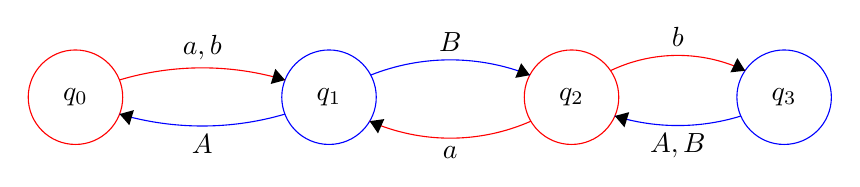
\begin{tikzpicture}[scale=0.2]
	\tikzstyle{every node}+=[inner sep=0pt]
	\draw [red] (13.5,-8) circle (3);
	\draw (13.5,-8) node {$q_0$};
	\draw [blue] (29.6,-8) circle (3);
	\draw (29.6,-8) node {$q_1$};
	\draw [red] (45,-8) circle (3);
	\draw (45,-8) node {$q_2$};
	\draw [blue] (58.5,-8) circle (3);
	\draw (58.5,-8) node {$q_3$};
	\draw [red] (16.29,-6.907) arc (106.6952:73.3048:18.309);
	\fill [black] (26.81,-6.91) -- (26.19,-6.2) -- (25.9,-7.16);
	\draw (21.55,-5.64) node [above] {$a,b$};
	\draw [blue] (32.245,-6.596) arc (111.67997:68.32003:13.685);
	\fill [black] (42.36,-6.6) -- (41.8,-5.84) -- (41.43,-6.77);
	\draw (37.3,-5.13) node [above] {$B$};
	\draw [blue] (26.802,-9.073) arc (-73.63011:-106.36989:18.635);
	\fill [black] (16.3,-9.07) -- (16.92,-9.78) -- (17.21,-8.82);
	\draw (21.55,-10.33) node [below] {$A$};
	\draw [red] (42.423,-9.522) arc (-66.20209:-113.79791:12.696);
	\fill [black] (32.18,-9.52) -- (32.71,-10.3) -- (33.11,-9.39);
	\draw (37.3,-11.1) node [below] {$a$};
	\draw [red] (47.469,-6.317) arc (115.60241:64.39759:9.906);
	\fill [black] (56.03,-6.32) -- (55.53,-5.52) -- (55.09,-6.42);
	\draw (51.75,-4.84) node [above] {$b$};
	\draw [blue] (55.755,-9.195) arc (-72.81583:-107.18417:13.556);
	\fill [black] (47.75,-9.19) -- (48.36,-9.91) -- (48.66,-8.95);
	\draw (51.75,-10.3) node [below] {$A,B$};
	\end{tikzpicture}
\end{center}

We say that states $q_0$ and $q_2$ are of kind $\Sigma_0 $, while $q_1$ and $q_3$ are of $\Sigma_1$. All edges coloured blue are of kind  $\Sigma_1 \rightarrow \Sigma_0$, and the red ones are $\Sigma_0 \rightarrow \Sigma_1$. 
Notice that formally, all states $q_0, q_1, q_2, q_3$ are of course of type $Q$. It's important to keep the distinction between kinds of states and types of mathematical objects. However, when you focus solely on kinds, you could think of a certain algebraic abstraction that forms a semigroup:
\begin{itemize}
	\item associate signs in alphabet with functions
	\item associate transitions/edges of automaton with members of those functions (keep in mind that a function could be defined as  set of pairs, so edges represent those exactly pairs)
	\item let function composition to be the semigroup operation
	\item then strings could be associated with compositions of those functions
	\item kinds of transitions in automaton become associated with types of those functions
\end{itemize}
\textcolor{red}{Tutaj mogę rozwinąć tą algebrę, lub mogę usunąć ten fragment i go nie poruszać. Nie jestem jeszcze pewien czy będzie to potrzebne do dowodów poprawności, chociaż wydaje się, że może bardzo pomóc.}

Notice that after erasing kinds, you are left with just 'plain' automaton that will work just fine as long as you don't feed it with invalid input (in the above example, input 'aAbBbBa' is valid, while  'aa', 'B' or 'aBB' are invalid). This is good news because we can reuse most of the algorithms for single-tape automaton and don't worry too much about generalising to multiple tapes. 

\paragraph{Multitape output} could be just as a useful feature as multitape input. However, this time we need a different approach. It makes little sense to have separate kind of states/edges for each output tape. We should be able to write to any tape, whenever we want. That's why cantor's pairing function is a way to go this time. 

\section{Correctness proofs}
\textcolor{red}{Podam dowody poprawności algorytmów przy pomocy wcześniej wprowadzonej aksojmatyzacji w logice Hoare'a} 

\end{document}
